\section{EVALUATION}
\label{chap:Evaluation}

To measure the effectiveness of dynamic windowing for multi-stream operators during the 
mapping of non-RDF heterogeneous data we need to measure the following 
metrics of our stream processing framework: \emph{CPU usage}, \emph{latency}, \emph{throughput},
\emph{memory usage}, and \emph{completeness}. 

\subsection{Data}
We use the same data 
as the benchmark in the paper by Van Dongen and Van den Poel~\cite{evalution_of_spe}. 
The data is provided by NDW (Nationale Databank Wegverkeersgegevens) from the 
Netherlands~\footnote{NDW data site: \href{http://opendata.ndw.nu/}{http://opendata.ndw.nu/} }.
It consists of measurements of the number of cars and their average speed across the different 
lanes on a highway. 
The sensor data was replayed by a Kafka publisher into two topics 
\emph{ndwflow} and \emph{ndwspeed}, for the number of cars and the average speed respectively.

\subsection{Evaluation setup}

Docker\footnote{Docker: \url{https://www.docker.com}} is 
setup with the containers 
as illustrated in Figure~\ref{fig:docker_setup}. The docker containers 
are run on a standalone machine in order to mitigate the influence of 
network communication as much as possible. Apache Kafka is used 
as the message broker for our data. The setup for the Kafka broker is 
the same as described in \cite{evalution_of_spe}. 



\begin{figure}[htpb]
    \centering
    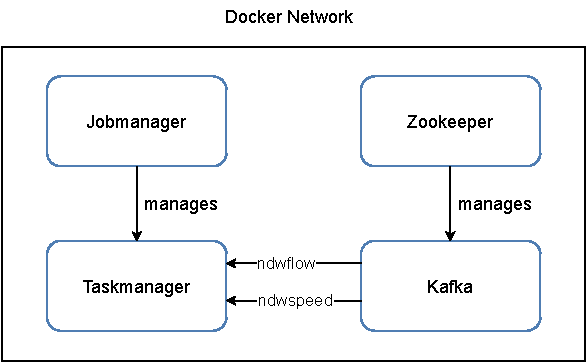
\includegraphics[width=\columnwidth]{fig/docker_setup.pdf}
    \caption[Setup of application containers inside the same docker network.]{ 
Setup of application containers inside the same docker network.
The kafka topics \emph{ndwflow} and \emph{ndwspeed} are consumed by the 
RMLStreamer job inside the Taskmanager.}
    \label{fig:docker_setup}
\end{figure}

\subsection{Metrics measurement}%
\label{sub:Metrics measurement}

CPU usage, throughput, memory, and latency exposed 
by Flink's Rest API, are constantly polled every 100ms by a 
Python script scraper.
CPU usage, throughput 
and memory usage are measured internally by Flink,
while latency measurement 
is implemented manually using Flink's Metrics API to more accurately measure the amount of 
time spent in the window by a record before being processed. 

The aforementioned metrics are averaged across the parallelized window operators.
Intersection over union (IOU) is used as the metric to measure the completeness
of the joined result generated by the windows.  


\subsubsection{CPU usage}%
\label{ssub:CPU usage}
For CPU usage, we measure Taskmanager's CPU usage, since it is 
the one responsible for executing the RMLStreamer code. 

\subsubsection{Throughput}%
\label{ssub:Throughput}
Throughput measurement is defined as the number of records processed by the 
window operator per second. 
It is measured at the output of the window operator, since we want to measure 
output performance of the window operators. 


\subsubsection{Memory usage}%
\label{ssub:Memory usage}
Due to limitation in granularity of measurement in Flink, 
JVM heap memory of the job is used to estimate the memory usage of window 
operator. We expect the memory usage by other operators in the job to be 
consistent and low across the different evaluation since they are stateless operators.

\subsubsection{Latency measurement}%
\label{ssub:Latency measurement}
We measure the latency by attaching a processing timestamp to the 
records before they enter the window. 
Once the records are processed and emitted after the join, the difference 
between the current processing time and the attached old processing time 
is taken as the \emph{latency} for the records. 

\subsubsection{Completeness measurement}%
\label{ssub:Completeness measurement}
To generate \emph{bounded} input data for 
the static mapping engine, we write the stored data from the topics 
into a file on disk. This input data is processed by RMLStreamer in bounded data 
processing mode to generate the \emph{complete} set of triples. 

The generated output triples from the evaluation of the windows, and the bounded data processing are 
used to calculate the IOU metric to measure the similarity between the two outputs.    



\subsection{Workload scenarios}
\label{sec:workload}
We evaluate our dynamic window implementation under different workload scenarios. 
These workloads are similar to the ones used in~\cite{evalution_of_spe} where relevant.

\subsubsection{Workload for latency measurement}
Measurement of the \emph{latency} caused only 
by the window implementations, requires the stream processing framework not to be 
stressed by significant \emph{throughput}. Thus, the Kafka broker 
publishes the records at a very low constant rate of around 400 messages per second for 
this workload. 

\subsubsection{Workload with periodic burst}
We evaluate our implementation for its ability to cope with unstable 
streaming data sources with varying velocity.
The workload has a constant low stream rate with an occasional 
burst of data. Therefore, 38 000 records will be published every 10 seconds which 
takes around 170ms to 180ms since the time taken to publish can deviate based on the 
load of the Kafka brokers. 

\subsubsection{Workload for completeness}
We will use two stream rates, constant and periodic, 
to measure the \emph{completeness} of the results generated 
by the different windows. The stream rates for constant and periodic are the same as their 
workloads previously mentioned. 






